\documentclass{article}
\usepackage{amsmath}
\usepackage{pgfplots}
\pgfplotsset{compat=1.16}

\begin{document}

\begin{figure}[h]
    \centering
    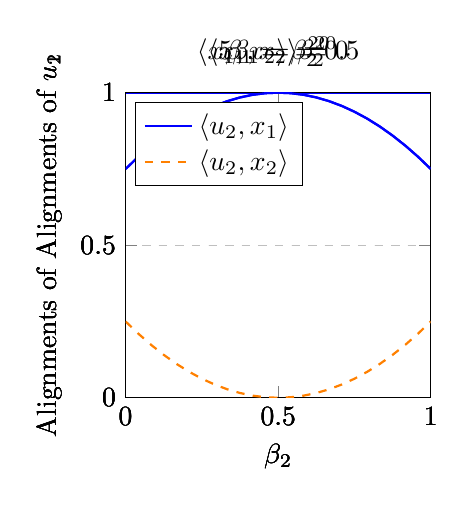
\begin{tikzpicture}
        \begin{axis}[
            xlabel=$\beta_{2}$,
            ylabel={Alignments of Alignments of $u_{1}$},
            xmin=0, xmax=1,
            ymin=0, ymax=1,
            xtick={0,0.5,1},
            ytick={0,0.5,1},
            legend pos=north west,
            ymajorgrids=true,
            grid style=dashed,
            title={$\langle x_{1},x_{2}\rangle = 0$},
            width=0.45\textwidth,
            height=0.45\textwidth,
            every axis plot/.append style={
                thick,
                mark options={mark size=1pt}
            }
        ]
            \addplot[blue, domain=0:1] {1};
            \addlegendentry{$\langle u_{1},x_{1}\rangle$}
            \addplot[orange, dashed, domain=0:1] {0};
            \addlegendentry{$\langle u_{1},x_{2}\rangle$}
        \end{axis}
        
        \begin{axis}[
            xlabel=$\beta_{2}$,
            ylabel={Alignments of Alignments of $u_{1}$},
            xmin=0, xmax=1,
            ymin=0, ymax=1,
            xtick={0,0.5,1},
            ytick={0,0.5,1},
            legend pos=north west,
            ymajorgrids=true,
            grid style=dashed,
            title={$\langle x_{1},x_{2}\rangle = 0.5$},
            width=0.45\textwidth,
            height=0.45\textwidth,
            every axis plot/.append style={
                thick,
                mark options={mark size=1pt}
            }
        ]
            \addplot[blue, domain=0:1] {1 - (x-0.5)^2};
            \addlegendentry{$\langle u_{1},x_{1}\rangle$}
            \addplot[orange, dashed, domain=0:1] {0};
            \addlegendentry{$\langle u_{1},x_{2}\rangle$}
        \end{axis}
        
        \begin{axis}[
            xlabel=$\beta_{2}$,
            ylabel={Alignments of Alignments of $u_{2}$},
            xmin=0, xmax=1,
            ymin=0, ymax=1,
            xtick={0,0.5,1},
            ytick={0,0.5,1},
            legend pos=north west,
            ymajorgrids=true,
            grid style=dashed,
            title={$\beta_{1}=\beta_{2}^{20}$},
            width=0.45\textwidth,
            height=0.45\textwidth,
            every axis plot/.append style={
                thick,
                mark options={mark size=1pt}
            }
        ]
            \addplot[blue, domain=0:1] {1};
            \addlegendentry{$\langle u_{2},x_{1}\rangle$}
            \addplot[orange, dashed, domain=0:1] {0};
            \addlegendentry{$\langle u_{2},x_{2}\rangle$}
        \end{axis}
        
        \begin{axis}[
            xlabel=$\beta_{2}$,
            ylabel={Alignments of Alignments of $u_{2}$},
            xmin=0, xmax=1,
            ymin=0, ymax=1,
            xtick={0,0.5,1},
            ytick={0,0.5,1},
            legend pos=north west,
            ymajorgrids=true,
            grid style=dashed,
            title={$5\beta_{1}=\beta_{2}^{20}$},
            width=0.45\textwidth,
            height=0.45\textwidth,
            every axis plot/.append style={
                thick,
                mark options={mark size=1pt}
            }
        ]
            \addplot[blue, domain=0:1] {1 - (x-0.5)^2};
            \addlegendentry{$\langle u_{2},x_{1}\rangle$}
            \addplot[orange, dashed, domain=0:1] {(x-0.5)^2};
            \addlegendentry{$\langle u_{2},x_{2}\rangle$}
        \end{axis}
    \end{tikzpicture}
    \caption{Sample figure showing different alignments of alignments.}
    \label{fig:sample_243}
\end{figure}

\end{document}